\documentclass[border=8pt]{standalone}
\usepackage{tikz}
\usetikzlibrary{positioning,arrows.meta,shapes.geometric,shapes.misc,fit,backgrounds}

\begin{document}
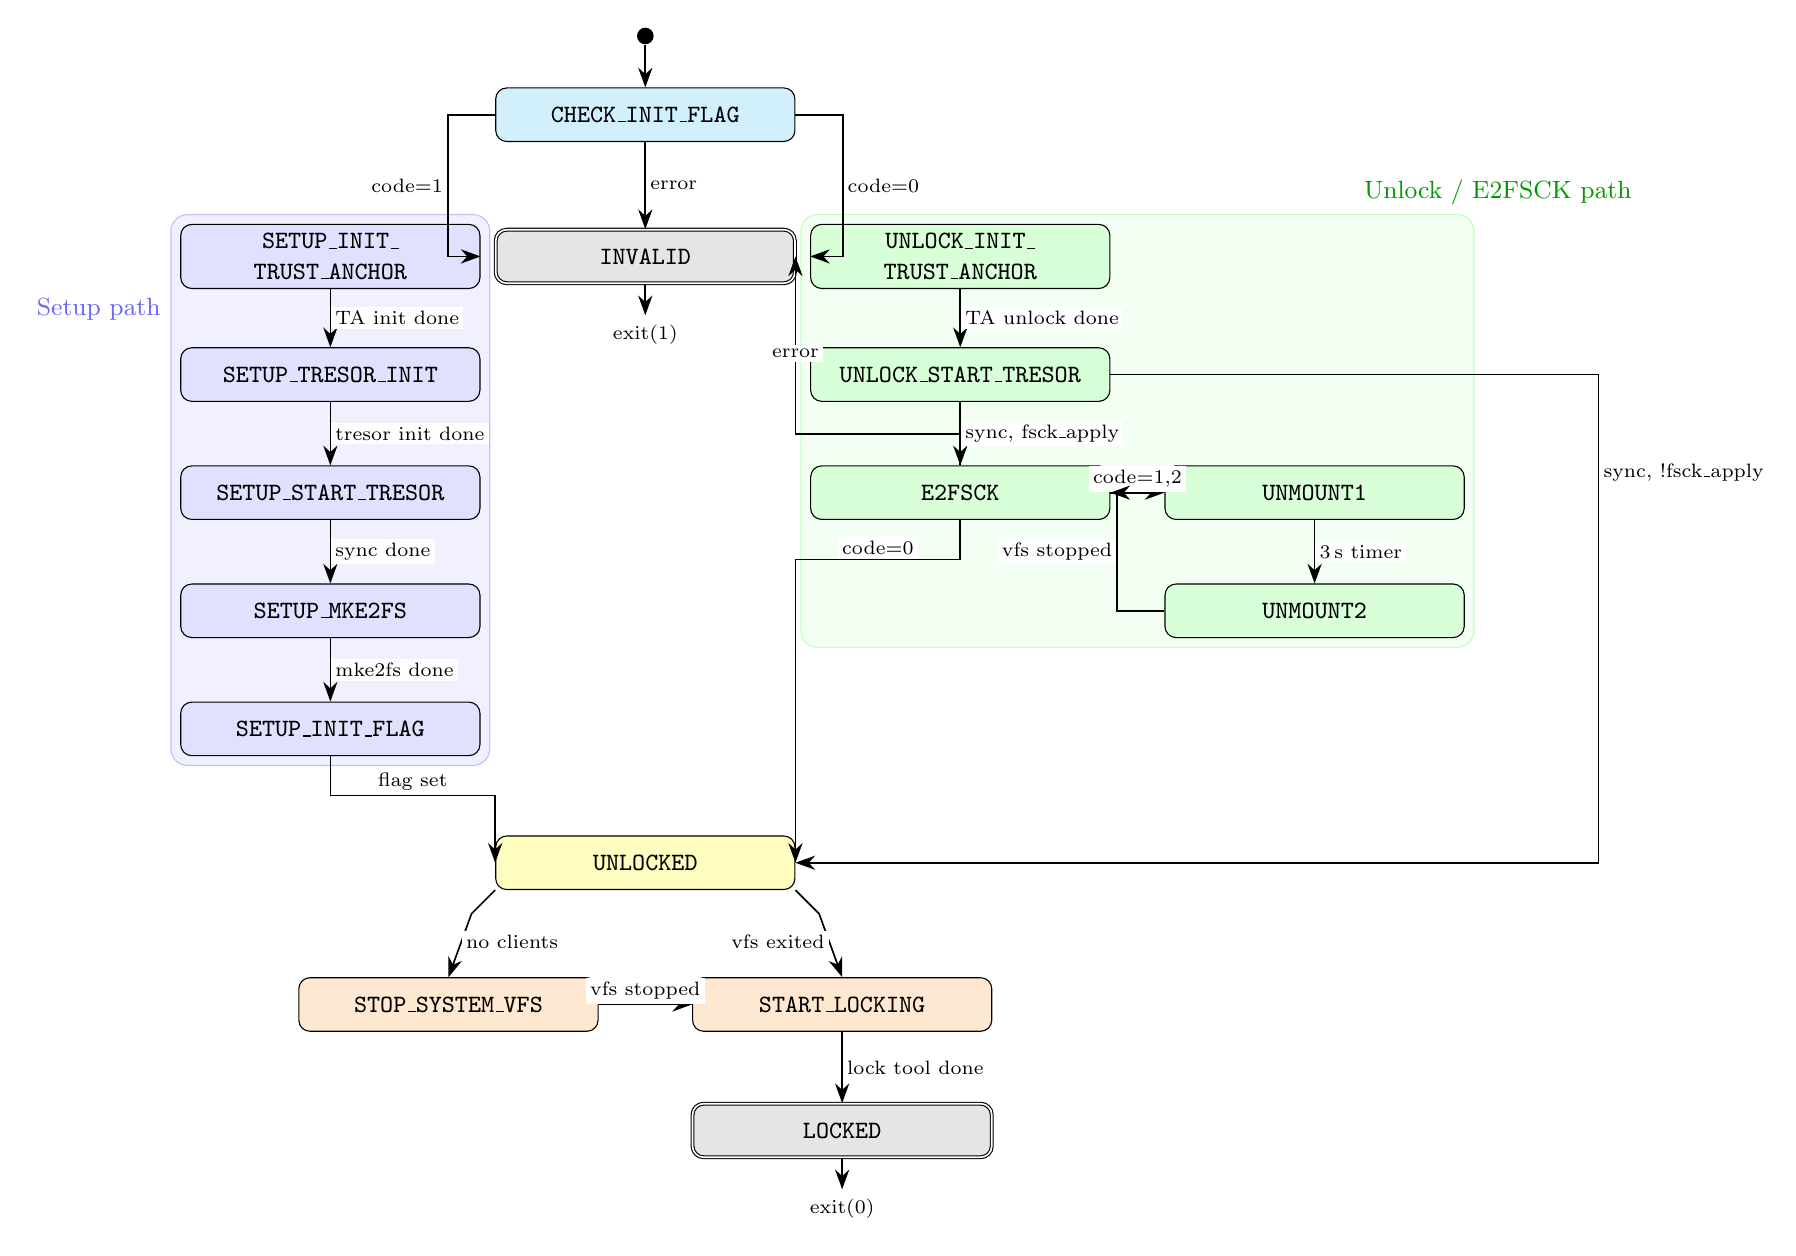
\begin{tikzpicture}[
  st/.style={draw, rectangle, rounded corners=4pt,
             minimum width=3.8cm, minimum height=0.68cm,
             align=center, font=\small\ttfamily},
  ssetup/.style={st, fill=blue!12},
  sunlock/.style={st, fill=green!15},
  sactive/.style={st, fill=yellow!25},
  slock/.style={st, fill=orange!18},
  sterm/.style={st, double, fill=gray!20},
  scheck/.style={st, fill=cyan!18},
  arr/.style={-{Stealth[length=2.5mm,width=1.8mm]}, semithick},
  lbl/.style={font=\scriptsize, fill=white, inner sep=1.5pt}
]

%% ── nodes ───────────────────────────────────────────────────────────────
\node[circle, fill=black, minimum size=6pt, inner sep=0] (dot)  at (4,  1.0) {};
\node[scheck]  (chk)   at (4,    0)    {CHECK\_INIT\_FLAG};
\node[sterm]   (inv)   at (4,   -1.8)  {INVALID};

%% Setup branch  (left column, x = 0)
\node[ssetup] (sta)   at (0,  -1.8)  {SETUP\_INIT\_\\ TRUST\_ANCHOR};
\node[ssetup] (sti)   at (0,  -3.3)  {SETUP\_TRESOR\_INIT};
\node[ssetup] (sst)   at (0,  -4.8)  {SETUP\_START\_TRESOR};
\node[ssetup] (smk)   at (0,  -6.3)  {SETUP\_MKE2FS};
\node[ssetup] (sif)   at (0,  -7.8)  {SETUP\_INIT\_FLAG};

%% Unlock branch (right column, x = 8)
\node[sunlock] (uta)  at (8,  -1.8)  {UNLOCK\_INIT\_\\ TRUST\_ANCHOR};
\node[sunlock] (ust)  at (8,  -3.3)  {UNLOCK\_START\_TRESOR};
\node[sunlock] (fsck) at (8,  -4.8)  {E2FSCK};

%% UNMOUNT cycle (far right, x = 12.5)
\node[sunlock] (um1)  at (12.5, -4.8)  {UNMOUNT1};
\node[sunlock] (um2)  at (12.5, -6.3)  {UNMOUNT2};

%% Convergence point
\node[sactive] (unl)  at (4,  -9.5)  {UNLOCKED};

%% Locking path
\node[slock]   (svfs) at (1.5,-11.3) {STOP\_SYSTEM\_VFS};
\node[slock]   (slk)  at (6.5,-11.3) {START\_LOCKING};
\node[sterm]   (lkd)  at (6.5,-12.9) {LOCKED};

%% ── edges ───────────────────────────────────────────────────────────────
% start arrow
\draw[arr] (dot) -- (chk);

% CHECK_INIT_FLAG
\draw[arr] (chk.west)  -- ++(-0.6,0)
           |- node[lbl,left,pos=0.25]{code=1}  (sta.east);
\draw[arr] (chk.east)  -- ++(0.6,0)
           |- node[lbl,right,pos=0.25]{code=0} (uta.west);
\draw[arr] (chk.south) -- node[lbl,right]{error} (inv.north);

% INVALID terminal
\draw[arr] (inv.south) -- ++(0,-0.4) node[below,font=\scriptsize]{exit(1)};

%% ─── Setup chain ─────────────────────────────────────────────────────────
\draw[arr] (sta) -- node[lbl,right]{TA init done}      (sti);
\draw[arr] (sti) -- node[lbl,right]{tresor init done}   (sst);
\draw[arr] (sst) -- node[lbl,right]{sync done}          (smk);
\draw[arr] (smk) -- node[lbl,right]{mke2fs done}        (sif);
% setup converges to UNLOCKED
\draw[arr] (sif.south) -- ++(0,-0.5)
           -| node[lbl,above,pos=0.25]{flag set} (unl.west);

%% ─── Unlock chain ────────────────────────────────────────────────────────
\draw[arr] (uta) -- node[lbl,right]{TA unlock done} (ust);
\draw[arr] (ust) -- node[lbl,right]{sync,\ fsck\_apply} (fsck);

% !fsck_apply bypass: go FAR RIGHT past UNMOUNT column, then down to UNLOCKED
\draw[arr] (ust.east) -- ++(6.2,0)    % x = 14.2
           |- node[lbl,right,pos=0.1]{sync,\ !fsck\_apply} (unl.east);

%% ─── E2FSCK ──────────────────────────────────────────────────────────────
\draw[arr] (fsck) -- node[lbl,above]{code=1,2} (um1);
\draw[arr] (um1)  -- node[lbl,right]{3\,s timer} (um2);
% UNMOUNT2 → E2FSCK: go left back
\draw[arr] (um2.west) -- ++(-0.6,0)
           |- node[lbl,left,pos=0.25]{vfs stopped} (fsck.east);

% E2FSCK code=0 → UNLOCKED
\draw[arr] (fsck.south) -- ++(0,-0.5)
           -| node[lbl,above,pos=0.25]{code=0} (unl.east);

% E2FSCK error → INVALID
\draw[arr] (fsck.north) -- ++(0,0.4)
           -| node[lbl,above,pos=0.7]{error} (inv.east);

%% ─── UNLOCKED ────────────────────────────────────────────────────────────
\draw[arr] (unl.south west) -- ++(-0.3,-0.3) -- (svfs.north)
           node[lbl,right,pos=0.45]{no clients};
\draw[arr] (unl.south east) -- ++(0.3,-0.3)  -- (slk.north)
           node[lbl,left,pos=0.45]{vfs exited};
\draw[arr] (svfs) -- node[lbl,above]{vfs stopped} (slk);
\draw[arr] (slk)  -- node[lbl,right]{lock tool done} (lkd);

% LOCKED terminal
\draw[arr] (lkd.south) -- ++(0,-0.4) node[below,font=\scriptsize]{exit(0)};

%% ── background group boxes ───────────────────────────────────────────────
\begin{scope}[on background layer]
  \node[rounded corners=6pt, fill=blue!6, draw=blue!25,
        fit=(sta)(sti)(sst)(smk)(sif),
        label={[font=\small,text=blue!60]above left:Setup path}] {};
  \node[rounded corners=6pt, fill=green!5, draw=green!25,
        fit=(uta)(ust)(fsck)(um1)(um2),
        label={[font=\small,text=green!60!black]above right:Unlock / E2FSCK path}] {};
\end{scope}

\end{tikzpicture}
\end{document}
